%%%%%%%%%%%%%%%%%%%%%%%%%%%%%%%%%%%%%%%%%%%%%%%%%%%%%%%%%%%%%%%%%%%%%%%%%%%%%%%
%
% Conclusion and outlook
% 
%%%%%%%%%%%%%%%%%%%%%%%%%%%%%%%%%%%%%%%%%%%%%%%%%%%%%%%%%%%%%%%%%%%%%%%%%%%%%%%
\chapter{Conclusion and outlook}
\label{cha6}

This final chapter concludes the thesis. First, we show the results of the application based on the presented data. Then a summary of the achievements and the resulting application is given in section \ref{sec6.2}. After that, section \ref{sec6.3} will present an outlook what future work could be done in this area. This also includes ideas or suggestions what should be changed or could be improved.

\section{Data tests}
In order to examine our application and to prove the efficiency of it, we want to run the application on several invoice documents. Using 300 invoice documents that each contain different company names, positions, values and layouts we have come to a conclusion to our work.

Before we present our results, we want to explain what has been measured and how we define \"accurate\".
There are multiple fields in an invoice document that are important for processing. To be able to provide the possibility to convert the document into an electronic invoice format we need to provide at least the following:
\begin{itemize}
\itemsep -1em 
	\item The invoice number
	\item The issue date
	\item The debitor (or as called in the ZUGFeRD specification: buyer)
	\item The creditor (or as called in the ZUGFeRD specification: seller)
	\item Line Total
	\item Charge Total
	\item Allowance Total
	\item Tax Basis Total
	\item Tax Total
	\item Grand Total
	\item The delivery date
\end{itemize}

We will calculate accuracy by counting all fields that have been found and are correct. This means every correct field will lead to an increased accuracy of $\frac{1}{11}$ in total. A processed document that leads to 11 correctly found fields will result to 100\% accuracy. 

As this application learns over time, we expect the accuracy to increase over time. Hence we will not only sum up the accuracy by using all results, but also show the accuracy evolution over time.

Figure \ref{accuracyTable} shows the resulting accuracy of the processed invoice documents: 
\begin{figure}[ht!]
\centering
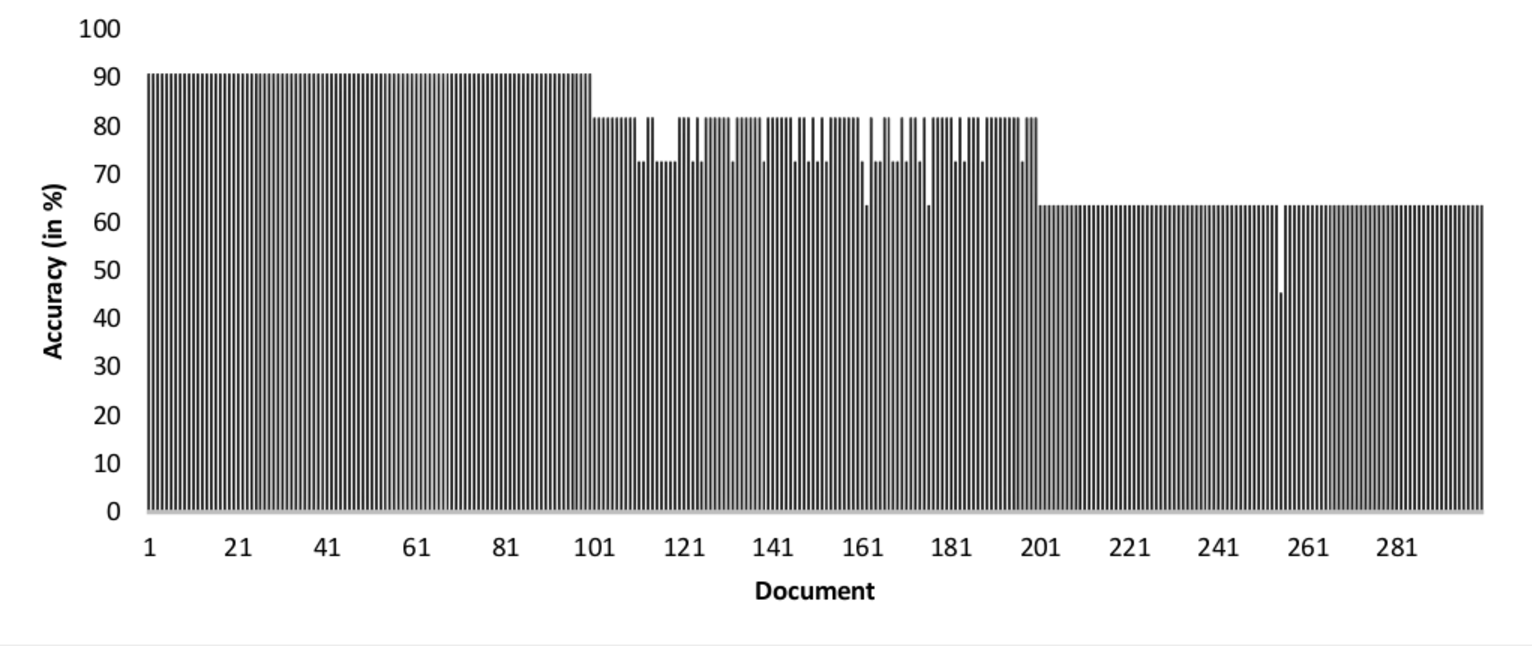
\includegraphics[width=\textwidth]{Images/Accuracy/Values.pdf}
\caption{Resulting accuracy of the application \label{accuracyTable}}
\end{figure}

There are especially two things that can be seen in this figure. First, the accuracy drops between the 100st and 200st document. This can be explained due to the fact that at this point another layout has been used. This also shows that the application is still dependent on the layout of the invoice document.

Secondly, the accuracy of the document processing is equal for each template (except some distortions). This indicates that our algorithm works data independently and its performance is mainly controlled by the document layout.

Eventually, we want to talk about the accuracy presented here. In all of the given invoices, there was always one information missing: The seller. This can be explained because of a missing learning step. In a normal case, the application would learn about a creditor the first time a document is processed. The next time, the application would be able to retrieve information of that creditor. Due to our automated testing approach, this step is missing. Hence there is missing information.
We took 10 documents of each layout and processed them manually in order to prove that explanation. Figure \ref{accuracyTable2} shows the accuracy compared to the previous one. Due to the information given to the application the new accuracy is higher than before.

\begin{figure}[ht!]
\centering
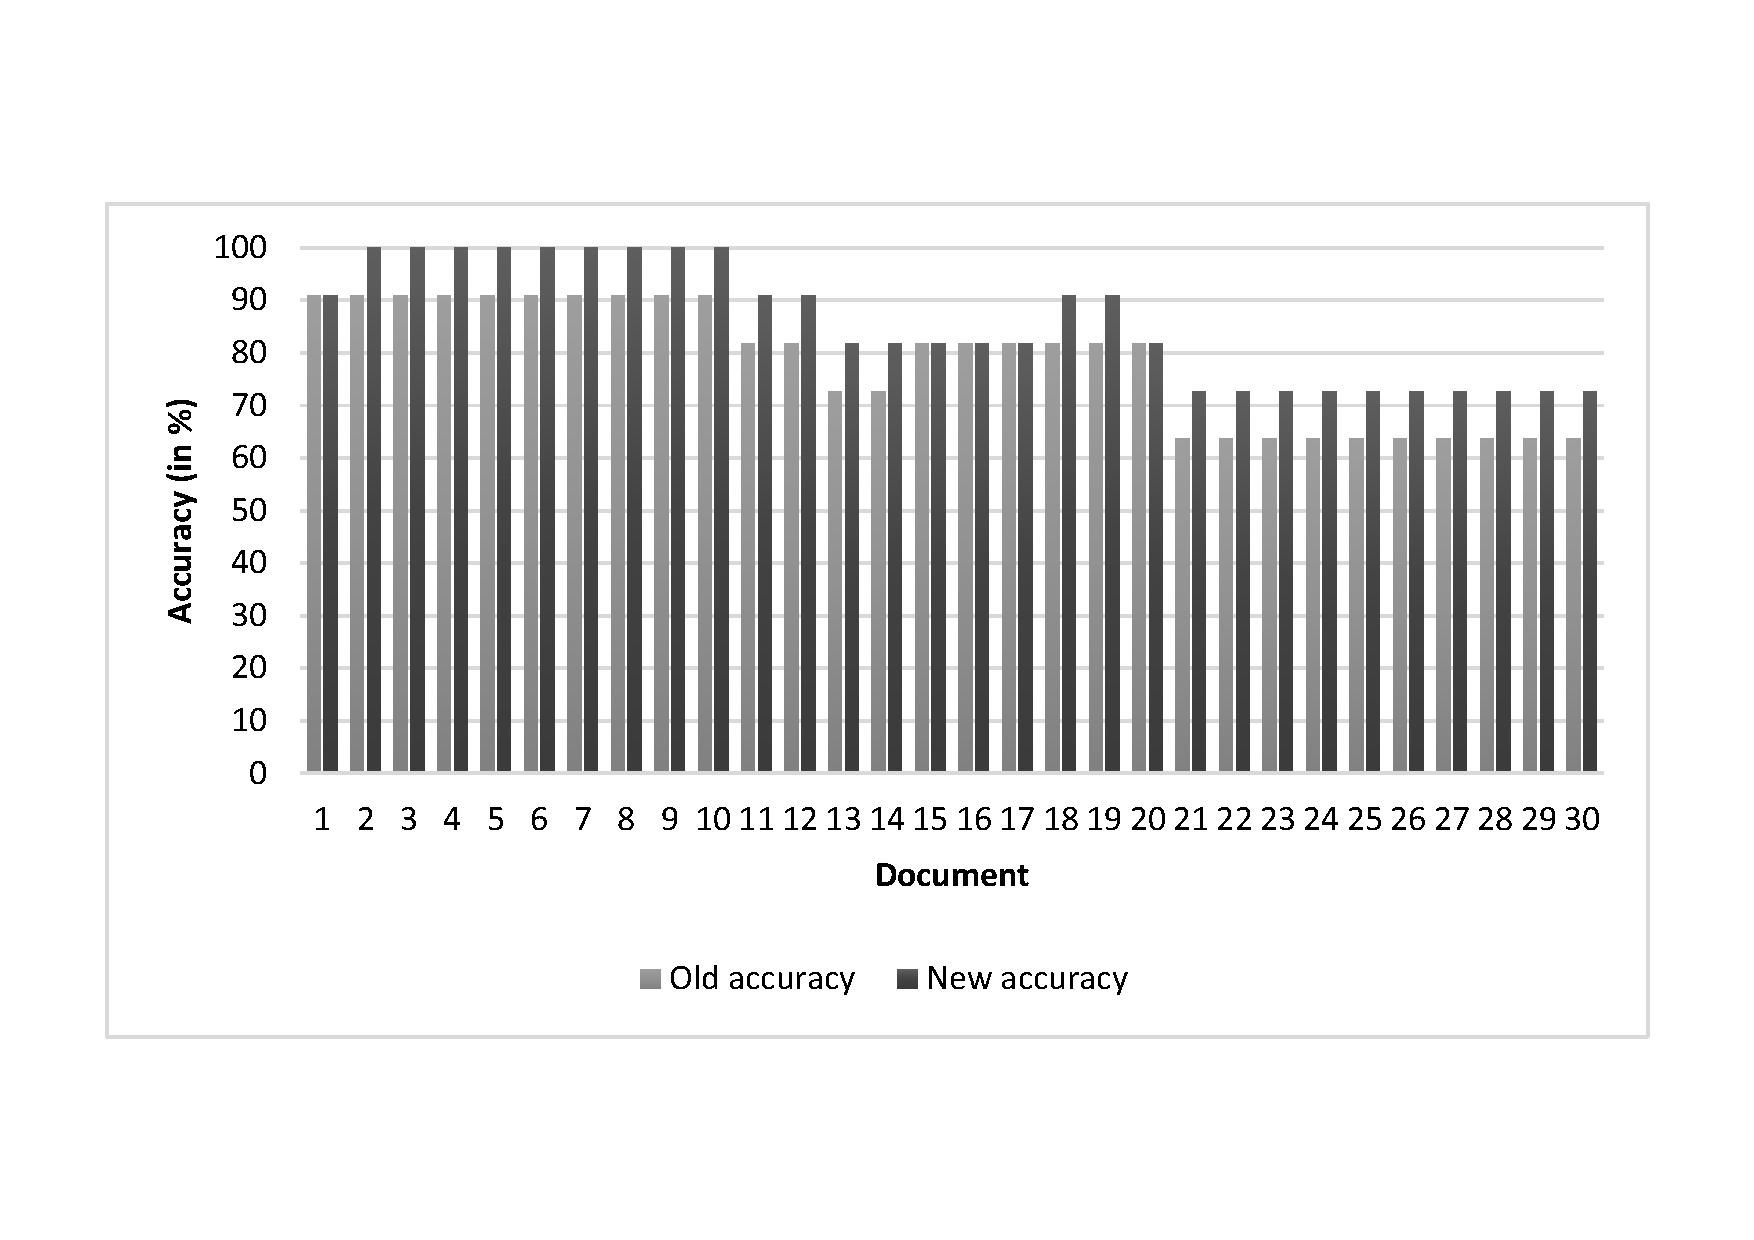
\includegraphics[width=\textwidth]{Images/Accuracy/Values2.pdf}
\caption{Resulting accuracy of the application \label{accuracyTable2}}
\end{figure}

This leads to the final presentation of the overall accuracy of the algorithm. Without the learning of a creditor, the application is able to process invoice documents with an accuracy of 77,81\%. After the application learned about the creditor, the accuracy increased to a value of 85,75\%.

\section{Conclusion}
\label{sec6.2}

The application presented in this thesis is capable of automatic form processing. Using OCR techniques, images and PDF documents can be scanned and words are extracted. The underlying OCR engine has been chosen by evaluating different products in order to select the most suitable one.
With implemented pre- and post-processing steps, the accuracy of the OCR has been enhanced. Using the hOCR format that has been presented by Thomas M. Breuel\cite{Breuel07}, position information of specific keywords are saved as cases. Those cases are used in order to improve the quality and accuracy of the algorithm over time. 

In addition to that, a Na{\"i}ve Bayes classificator is used to learn possible ways of accounting a position in regards to the possible accounting strategies different users (or companies) can apply on the same position. The selection of a machine learning classifier has been made by evaluating different approaches and their accuracy. 

As proposed in 2014, a new electronic invoice format - ZUGFeRD - has been published which has a high future potential\cite{Ferd14}. This standard is not only already used by the German state administration but is also conform with the EU directive 2014/55/EU that plans a European-wide mandatory implementation of such a standard for all state administrations. 
ZUGFeRD is supported by the application, as the result of the processing will be a full conformal invoice of this scheme. The support of this format is a result of a comparison between leading and potential interesting formats in the future and the decision using predefined criteria.

The resulting converted invoices are stored in a MySQL database and can be retrieved by the user. Additional filtering allows a facilitated retrieval process. This process is also secure against SQL injections.

Several parameters of the application are customized and enable adjustments and personal preferences of the user. This also allows to further define the minimum confidence the application should have in regards to an invoice document as it classifies the document based on the confidence level. 

\section{Future Work}
\label{sec6.3}
Even though the application is finalized and working, several improvements could be made in the future.
Each of them will be listed here, including the reasons why they should be made as well as possible ideas on how to achieve these improvements.

Improving the accuracy of OCR: As the application is highly dependent on the successful and accurate process of OCR, improving the accuracy of the OCR process will improve the usefulness of this application in general. Hence, every action made in this direction is an advantage. There are two ideas that could be realized in the future: 
	\begin{itemize}
		\item Improving the accuracy of the Tesseract by creating an own training set based on a representative amount of invoices (especially in German) of different companies. 
		\item Exchanging the open source solution for a proprietary solution that provides a higher accuracy and / or is specialized either on invoices or German text.
	\end{itemize}

Refactor the overall design of the application: Various adjustments in the application could be made to make the application more extensible in the future. The following is a list of possible changes:
	\begin{itemize}
		\item Using the strategy pattern on the OCR module: The application should be independent from which kind of OCR API it retrieves the String output. The strategy pattern would ideally lead to the possibility for the user to choose the preferred OCR reader from the settings view.
		\item Removing unnecessary or unused Business Objects, such as the Address or CorporateForm classes, since those are not used at the moment. Or instead, extend the application to make use of those classes.
	\end{itemize}

Increase the performance of the processing step: The slowest part of the application is the process of scanning a document and extracting its information. Finding a way to speed-up this step would lead to a faster application. One idea would be to parallelize the process of information retrieval with multiple documents and make use of all processor cores the device the application runs on has.

Add support for other electronic invoice standards: As of now, the application only supports the ZUGFeRD standard. But as stated in section \ref{sec2.3.2} before, EDIFACT has a high future potential. This also applies to the UBL standard. The more standards this application supports, the more companies can make use of it.

While comparing positions we could make use of a wordnet implementation that enables us to find similar words. This way we would be able to interpret the position string in a semantic way.

Supporting other account systems besides the SKR03 could lead to a higher usefulness for companies using other account systems (such as the SKR04).